\renewcommand{\thesubsection}{\textcolor{red}{\Roman{section}.\arabic{subsection}}}
\renewcommand{\thesubsubsection}{\textcolor{red}{\Roman{section}.\arabic{subsection}.\alph{subsubsection}}}

\setcounter{section}{0}
\setcounter{document}{0}
\sndEnTeteDMUn

\begin{center}
\begin{mdframed}[style=titr, leftmargin=60pt, rightmargin=60pt, innertopmargin=7pt, innerbottommargin=7pt, innerrightmargin=8pt, innerleftmargin=8pt]

\begin{center}
\large{\textbf{Devoir maison 1 : la composition de l'air}}
\end{center}

\end{mdframed}
\end{center}

\begin{wrapfigure}{r}{0.3\textwidth}
\vspace{-1cm}
    \centering
      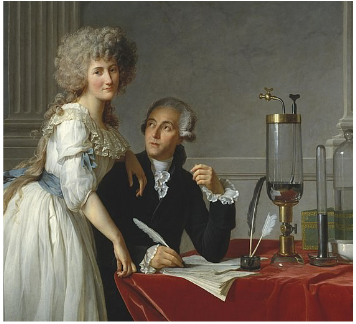
\includegraphics[width=0.3\textwidth]{Images/Activite_1/Lavoisier.png}
  \end{wrapfigure}
Antoine Laurent Lavoisier (1743-1794) est considéré comme le père de la chimie moderne. Avec ses multiples expériences sur l’air, le dioxygène, ou le dioxyde de carbone, il montre que la matière est
constituée d’espèces chimiques (même s’il n’emploie pas ce terme), et non de quatre éléments (feu, terre, eau et air) comme les anciens chimistes
l’admettaient.\\
\newline

\begin{doc}{Lecture d'un volume sur la verrerie}
\begin{wrapfigure}{r}{0.2\textwidth}
\vspace{-1cm}
    \centering
      
\includegraphics[width=0.2\textwidth]{Images/DM/Qr_code_Lavoisier.png}
  \end{wrapfigure}
En 1775, Antoine Lavoisier réalise une expérience qui lui permet de déterminer la composition de l’air.
Son expérience est résumée dans la vidéo suivante : \url{https://ladigitale.dev/digiplay/#/v/6305f2f7b8fd4}.\\
D’après Lavoisier, l’air est constitué de deux gaz : le dioxygène et le diazote. Le volume du gaz initialement
présent dans la cloche est de 0,80 L d’air. À la fin de l’expérience, le volume du gaz qui n’a pas réagi avec le
mercure (c’est-à-dire le diazote) est de 0,66 L.
\end{doc}

\begin{doc}{Proportion volumique ou massique d’une espèce dans un mélange}
Pour décrire la composition d’un mélange, on indique la proportion (ou le pourcentage) de chaque espèce chimique constituant le mélange. On peut choisir d’utiliser la proportion massique notée $x_m$, ou la proportion volumique notée $x_V$ :
\begin{align*}
    x_m &= \frac{m_{\text{espèce}}}{m_{\text{totale}}} & x_V & = \frac{V_{\text{espèce}}}{V_{\text{totale}}}\\
\end{align*}
Ces deux grandeurs s'expriment en général en \%.
\end{doc}

\begin{doc}{Données utiles}
On donne les informations suivantes à pression atmosphérique :
\begin{itemize}
    \item 1 mL de dioxygène a une masse $m_{O_2}
=1,354$~mg à $15\degreCelsius$,
    \item 1 mL de diazote a une masse $m_{N_2}
=1,185$~mg à $15\degreCelsius$,
    \item 1 mL d’air ambiant a une masse $m_{air}=1,225$~mg à $15\degreCelsius$.
\end{itemize}
\end{doc}

\newpage

\question{Résumer en quelques lignes l’expérience de Lavoisier}{Lavoisier fait chauffer un récipient (un matras) rempli de mercure qui est relié à une cloche remplie d'air placée dans une bassine d'eau servant à mesurer le volume d'eau. Le mercure réagit avec le dioxygène présent de la cloche formant un précipité d'oxyde de mercure \chemform{HgO}. Le volume qu'occupe le gaz dans la cloche a donc varier et Lavoisier peut en déduire la proportion de chaque espèce présente dans l'air.}{4}
\\
\question{Déterminer si l’air est un corps pur, un mélange homogène ou un mélange hétérogène. Justifier.}{D'après le document 1, l'air est constitué d'au moins deux gaz différents : le dioxygène \chemform{O_2}, le diazote \chemform{N_2}. Il s'agit donc d'un mélange (ici gazeux). On ne distingue pas les deux gaz à l'\oe il nu. L'air est donc un mélange homogène.}{2}
\\
\question{Calculer la proportion volumique de diazote dans l’air obtenue d'après l'expérience de Lavoisier.}{D'après le document 1, le volume de diazote n'ayant pas réagi avec le mercure vaut $V_{N_2}=0,66$~L. Le volume total de gaz initialement présent dans la cloche était de $V_{tot}=0,80$~L. On en déduit la proportion volumique de \chemform{N_2} d'après la formule donnée par le document 3 : \begin{equation*}
    x_{V}(N_2)\frac{V_{N_2}}{V_{tot}}=\frac{0,66}{0,80} = 0,83 = 83\%
\end{equation*}}{2}
\\
\question{Déduire de la question précédente le volume initial du dioxygène. Quelle était la masse initiale $m_{O_2}(ini)$ de dioxygène dans l'expérience de Lavoisier ?}{On déduit de la proportion volumique de diazote de la question précédente la proportion volumique de dioxygène :
\begin{equation*}
    x_V(O_2) =1-x_V(N_2) = 17\%
\end{equation*}
On en déduit le volume initial de dioxygène par rapport au volume total de la cloche $V_{tot}=0.80$~L :
\begin{equation*}
    V(O_2)=x_V(O_2)\times V_{tot}=0,17\times 0,80 = 0,14~\text{L} = 140~\text{mL}
\end{equation*}
Remarque : ce résultat est bien sur cohérent avec les données du document 1 : $V(O_2)=V_{tot}-V(N_2)=0,80-0,66=0,14$~L.\\
On en déduit la masse de \chemform{O_2} d'après les données du document 3 :
\begin{equation*}
    m_{O_2}(ini)=1,354~\text{g/mL}\times\underbrace{140~\text{mL}}_{\text{Attention aux unités !}} = 190~\text{mg}
\end{equation*}}{5}

\question{À présent, calculer la proportion massique de diazote dans l’air et la proportion massique de dioxygène dans l’air. Les valeurs sont-elles exactement les mêmes que celles de la figure 2 du Chapitre 1 ? A votre avis, pourquoi ?}{Même calcul que précédemment :
\begin{equation*}
    m_{N_2}(ini)=1,185~\text{g/mL}\times 660~\text{mL} = 782~\text{mg}
    \end{equation*}
La masse totale d'air est $m_{tot}=1,225~\text{g/mL}\times 800~\text{mL}=980$~mg. Les proportions massiques du dioxgène et de diazote sont donc :
\begin{align*}
    x_m(O_2) &= \frac{190}{980} = 0,19\% & x_m(N_2) = \frac{782}{980} = 0,80\%
\end{align*}
On peut faire les hypothèses quant aux écarts avec la figure 2 :
\begin{itemize}
    \item erreurs de lecture du volume dans l'expérience,
    \item les données du document 3 sont pour une température de 15$\degreCelsius$, dans l'expérience la température pouvait être différente (certainement puisqu'on chauffe du mercure). 
\end{itemize}}{5}